\documentclass[Bachelorarbeit.tex]{subfiles}
%to translate single chapters
%	comment out first line
%	insert following two lines
%\documentclass[a4paper,12pt]{report}
%\usepackage{../sty/fhv}

\begin{document}
\chapter{Problem description}\label{ProblemDescription}
\section{Overview}
According to the articel \cite{FRLiteratureSurvey} face recognition can be segmented into three key steps, shown in figure \ref{FRP}.

\begin{figure}[hbtp]
\centering
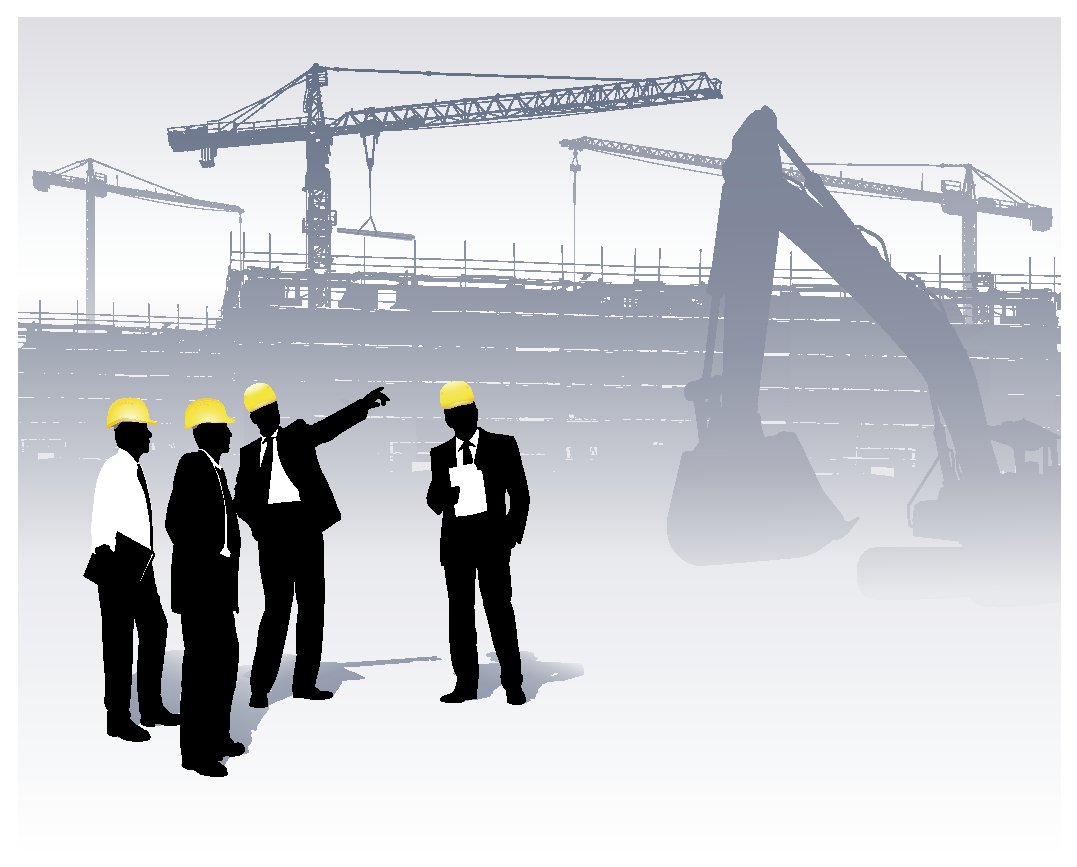
\includegraphics[width=8cm]{./pictures/UnderConstruction}
\caption{Face Recognition Progress \label{FRP}}
\end{figure}

\textbf{Face Detection} is responsible for a rough normalization (like face tracking) and use for this task different approaches (see figure \ref{FDa}).\\
\textbf{Face Extraction} generates a more accurate normalization (like human emotions). The different approaches to get this emotions are shown in figure \ref{FEa}. Face detection and face extraction approaches can use the same feature-based-method (like informations out of color, Motion, ... see figure \label{FDaSurvey}) so they can perform simultaneous. \\
\textbf{Face Recognition} is the last step to identify/verify a picture. For a verification/identification several methods (see figure \ref{FRa}) are available.


\begin{figure}[!h] %Face Detection Approach
\centering
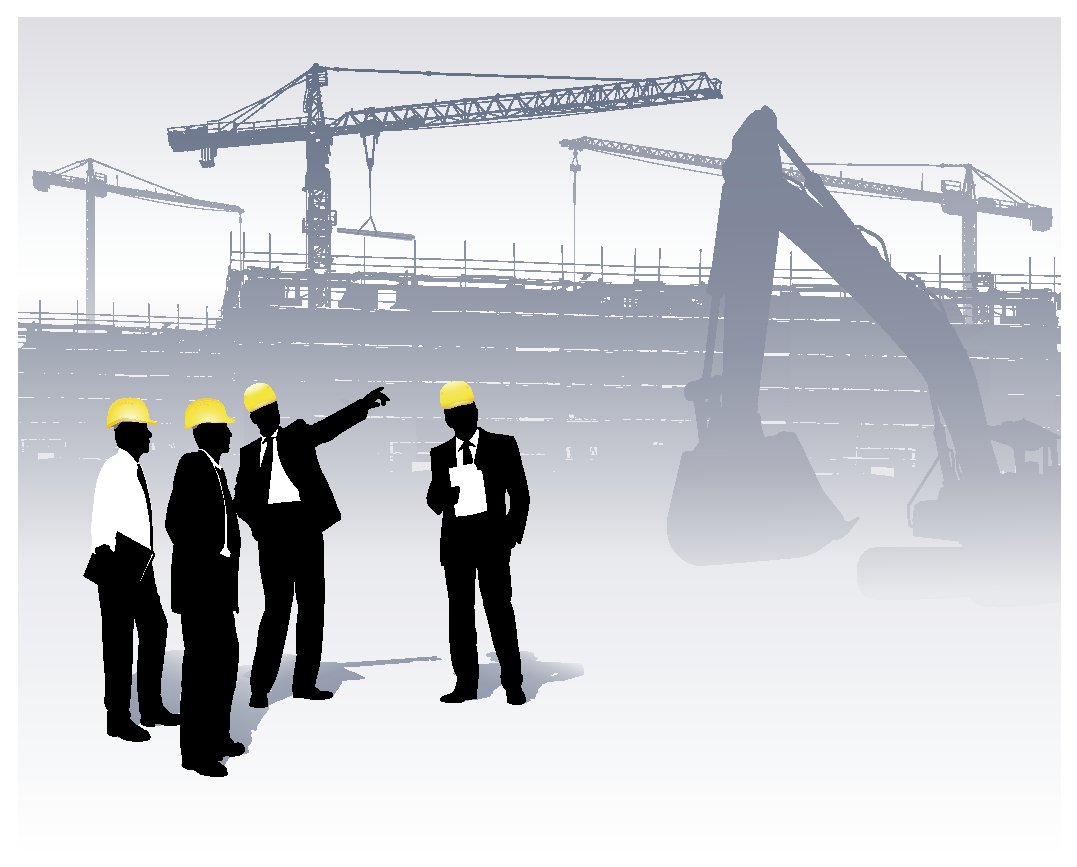
\includegraphics[width=5cm]{./pictures/UnderConstruction}
\caption{Face Detection divided into approaches. \label{FDa}}
\end{figure}

\begin{figure}[!h] %Face Extraction Approach
\centering
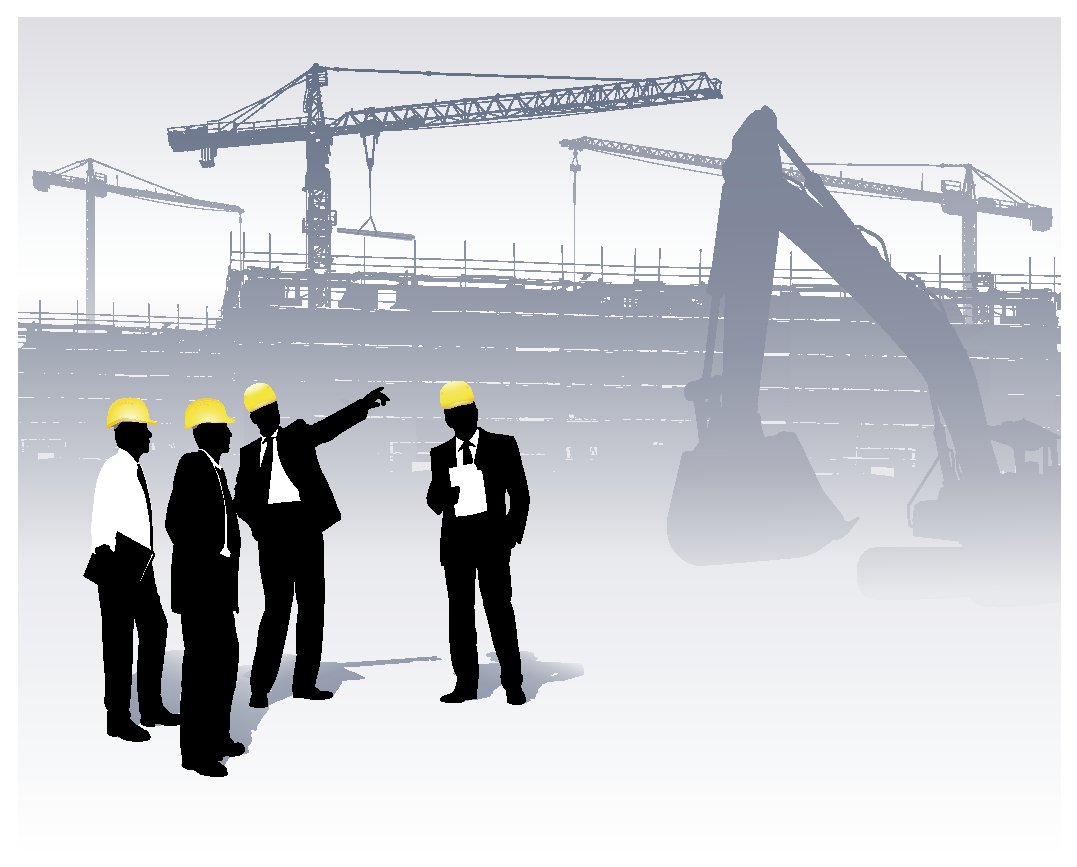
\includegraphics[width=5cm]{./pictures/UnderConstruction}
\caption{Face Extraction divided into approaches. \label{FEa}}
\end{figure}

\begin{figure}[!h] %Face Recognition Approach
\centering
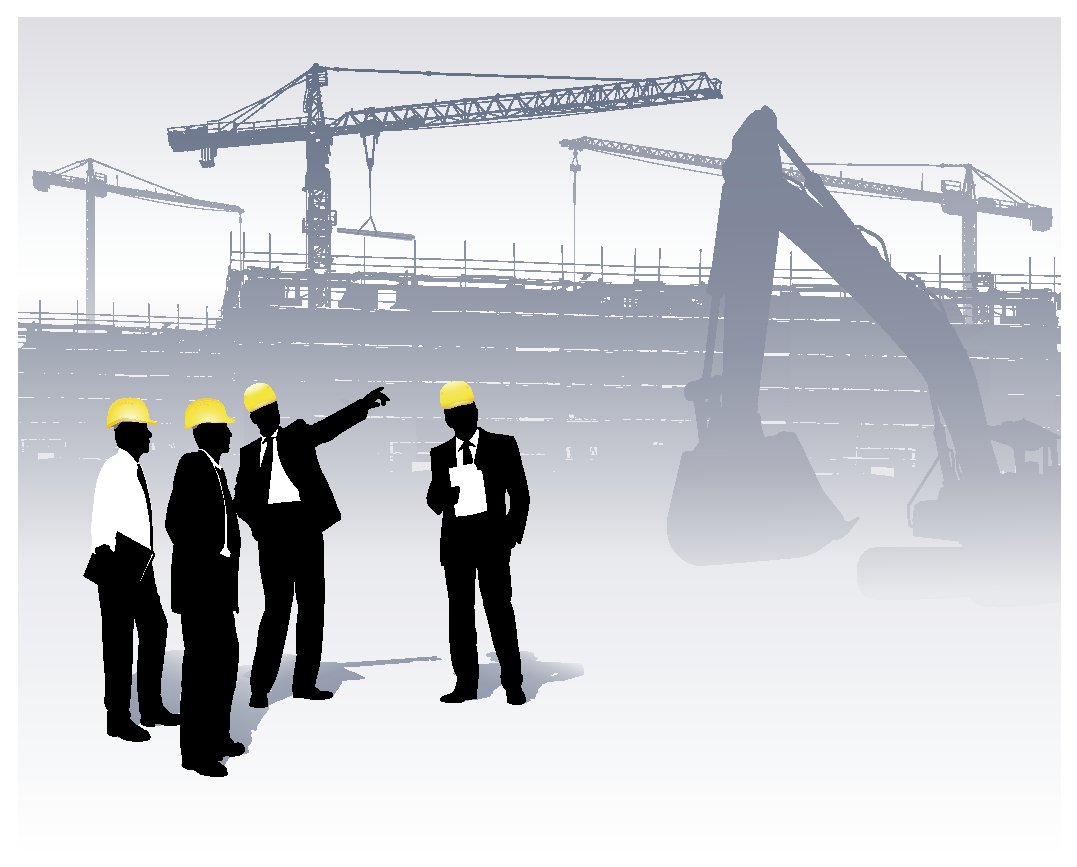
\includegraphics[width=5cm]{./pictures/UnderConstruction}
\caption{Face Recogntition divided into approaches. \label{FRa}}
\end{figure}

\section{Face Detection}
The most interest part from our point of view was the Face detection. To find an approach which we can study, implement and test we made further researches in this segment. The article \cite{FDASurvey} gives a good overview of the topic face detection. The figure \ref{FDaS} (out of \cite{FDASurvey}) represents the different approaches to detect faces in a picture.

\begin{figure}[!h] %Face Detection detaild approaches
\centering
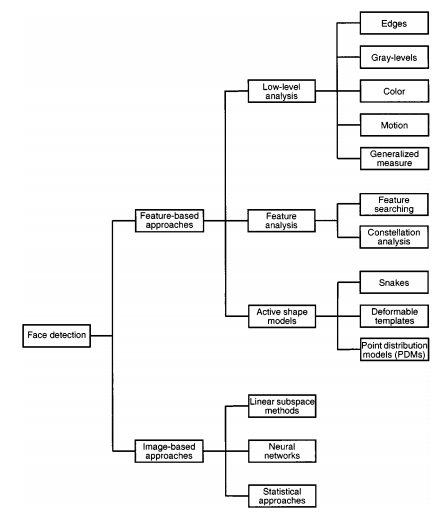
\includegraphics[width=10cm]{./pictures/FaceDetectionApproaches}
\caption{Face Detection divided into approaches (more detailed). \label{FDaS}}
\end{figure}

The most interesting approach for us was \textit{Face detection based on color likelihood} approach (in figure \ref{FDaS} marked as \textit{Color}).


\end{document}
